\section{Proposed Methods}
\label{sec:slam-methodology}

The following subsections describe the methods developed and integrated to achieve globally consistent, ENU-referenced localisation in vineyard environments. These contributions build on the GLIM framework surveyed in the preceding section and address the key challenges of reference frame alignment, GNSS outlier rejection, and parameter optimisation.

To begin this investigation, we implemented GLIM \cite{koideGLIM3DRangeInertial2024}. We chose GLIM as it had infrastructure in place to add extension modules to incorporate new sensors and capabilities. GLIM provides a global callback slot mechanism that allows access to the internal states of the mapping process and insertion of additional constraints into the factor graph. GLIM also eliminated sensor-specific processes, meaning it can be applied to a wide variety of range sensors such as spinning-type LiDAR, non-repetitive scan LiDAR, solid-state LiDAR and even RGB-D cameras.

GLIM state estimation is created in the local odometry frame. For our use in the wider research project, we required state estimation in the local ENU reference frame, which is a surveyed-in point at each of our farms. Thus, we needed a procedure to align the GLIM reference frame with the existing local ENU reference frame.

Firstly, we time synchronise the on-board GPS unit with the LiDAR and with the system clock. This allows us to associate corresponding GNSS points with the submaps or keyframes of LiDAR frames that GLIM registers, as illustrated in \cref{fig:time-matching}. We aggregate a set of corresponding GNSS coordinates with keyframe coordinates, and then implement the Kabsch algorithm \cite{kabschSolutionBestRotation1976} to find the relative transform between the two point sets by minimising the root-mean-square deviation between the two point sets.

\begin{figure}[htbp]
    \centering
    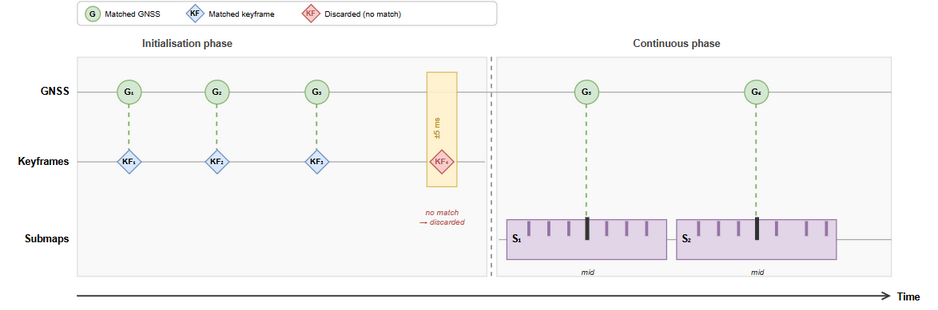
\includegraphics[width=\linewidth]{3-SLAM/3-methodology/figures/time-matching}
    \caption{GNSS-to-frame time matching across both operating phases. During the initialisation phase, each keyframe (KF) is matched to a GNSS measurement within a $\pm5$\,ms window enforced by PTP/Chrony clock synchronisation. A keyframe with no GNSS measurement in its window is discarded. During the continuous phase, submaps are matched using the timestamp of their middle keyframe (\textit{mid}), which approximates the temporal centroid of the submap.}
    \label{fig:time-matching}
\end{figure}

The Kabsch algorithm relies on the least-squares method to minimise the root-mean-square deviation (RMSD) between two point sets. Since the objective function squares the distances between paired points, outliers produce disproportionately large influences on the final transformation matrix. Thus, for global alignment, it is important that outliers are filtered out before executing the Kabsch algorithm. \cref{fig:system-pipeline} illustrates the complete proposed pipeline from sensor input to globally consistent ENU trajectory output.

\begin{figure}[htbp]
    \centering
    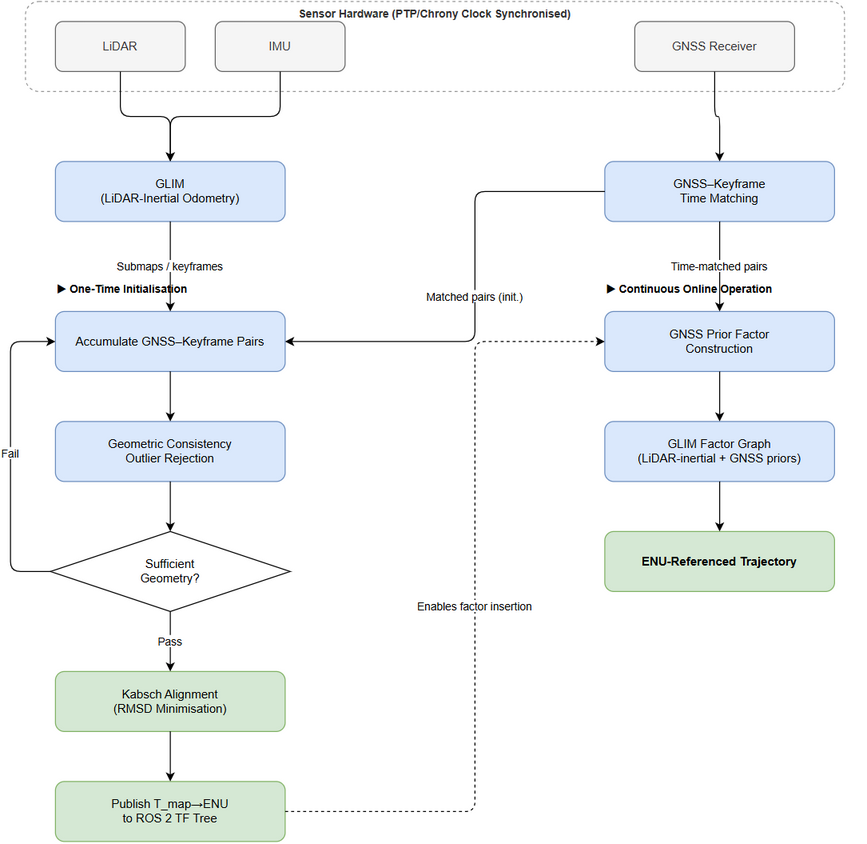
\includegraphics[width=\linewidth]{3-SLAM/3-methodology/figures/system-pipeline}
    \caption{Overview of the proposed GNSS-augmented SLAM pipeline. The initialisation track (left) performs time synchronisation, outlier rejection, planar geometry quality assessment, and Kabsch alignment to publish the map-to-ENU transform. The continuous track (right) constructs GNSS prior factors and inserts them into the GLIM factor graph for ongoing drift correction. On geometry check failure, initialisation waits and accumulates further GNSS--pose correspondences before retrying.}
    \label{fig:system-pipeline}
\end{figure}

\subsection{Geometric Consistency-Based Outlier Rejection}

To remove spurious GNSS measurements prior to initialisation, we apply a geometric consistency check that exploits the rigidity of the GNSS--IMU transformation. The method assumes that, for inlier measurements, pairwise distances between GNSS observations should be preserved when mapped into the local map frame via the estimated poses.

Let $\{\mathbf{g}_i\}_{i=1}^{N}$ denote GNSS positions expressed in the ENU frame, and $\{\hat{\mathbf{g}}_i\}_{i=1}^{N}$ denote the corresponding GNSS positions expressed in the map frame, obtained by transforming IMU poses with a fixed extrinsic calibration. For each point $i$, we evaluate its consistency with all other points $j \neq i$ by comparing pairwise Euclidean distances in both frames as shown in Equation \eqref{eq:consistency_check}:
\begin{equation}
\label{eq:consistency_check}
\left| \lVert \mathbf{g}_i - \mathbf{g}_j \rVert - \lVert \hat{\mathbf{g}}_i - \hat{\mathbf{g}}_j \rVert \right| < \tau,
\end{equation}
where $\tau$ is a distance consistency threshold reflecting accepted SLAM error and GNSS noise.

This approach was chosen over stochastic methods like RANSAC \cite{fischlerRandomSampleConsensus1981} or iterative M-estimators because it takes advantage of the invariance of pairwise Euclidean distances under rigid body transformations, which means that the method remains entirely deterministic and independent of any initial pose estimate or probabilistic modelling.

To formalise the inlier classification, we define a pairwise consistency indicator $c_{ij}$ in Equation \eqref{eq:indicator}:
\begin{equation}
\label{eq:indicator}
c_{ij} = 
\begin{cases} 
1 & \text{if } \left| \lVert \mathbf{g}_i - \mathbf{g}_j \rVert - \lVert \hat{\mathbf{g}}_i - \hat{\mathbf{g}}_j \rVert \right| < \tau \\
0 & \text{otherwise}
\end{cases}
\end{equation}
A measurement is classified as an inlier if the fraction of other points with which it satisfies the above constraint exceeds a minimum inlier ratio $\rho$, satisfying the condition:
\begin{equation}
\label{eq:majority_criterion}
\frac{1}{N-1} \sum_{j \neq i}^{N} c_{ij} > \rho.
\end{equation}

GNSS multipath errors \cite{wenExclusionGNSSNLOS2018} can often create erroneous clusters of points that are mutually consistent, and therefore are not filtered out by conventional statistical outlier methods. However, the majority-based criterion in Equation \eqref{eq:majority_criterion} ensures that points are only kept if they belong to the global rigid consensus, effectively filtering out clusters of mutually consistent but globally erroneous points. After classification, only inlier GNSS measurements and their corresponding map-frame estimates are preserved for subsequent processing. \cref{fig:outlier-rejection} illustrates a representative scenario in which inlier measurements lie along the physical trajectory while a multipath cluster is correctly rejected.

\begin{figure}[htbp]
    \centering
    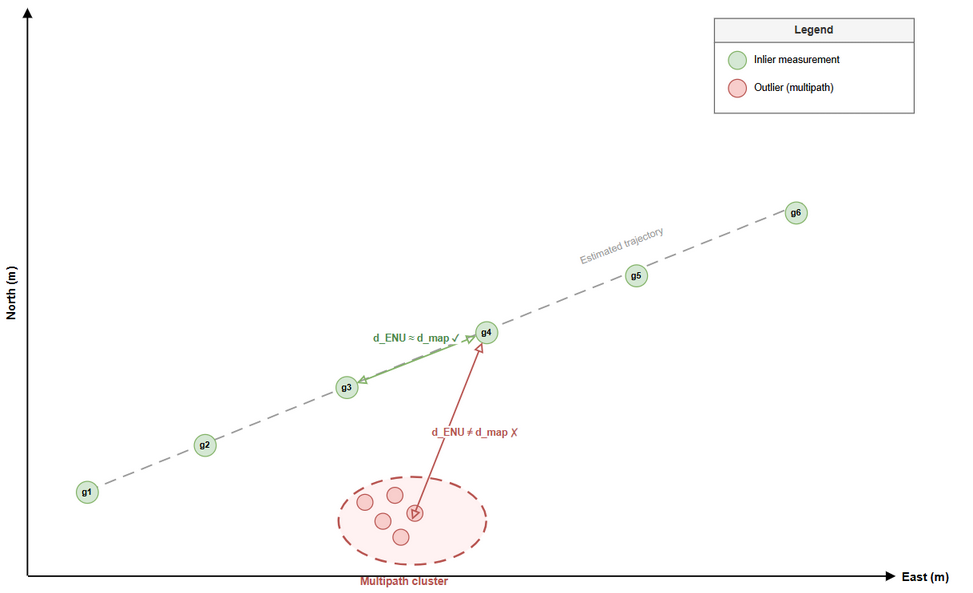
\includegraphics[width=0.75\linewidth]{3-SLAM/3-methodology/figures/outlier-rejection}
    \caption{Geometric consistency-based outlier rejection applied to GNSS measurements. Inlier points (green) are distributed along the estimated trajectory and satisfy pairwise distance consistency with map-frame estimates. Multipath-corrupted points (red) form a spatially compact cluster that is globally inconsistent with the rigid consensus and are therefore rejected, even though they are mutually self-consistent.}
    \label{fig:outlier-rejection}
\end{figure}

\subsection{Planar Geometry Quality Assessment in 2D}

Subsequently to outlier rejection, we assess the geometric quality of the remaining point set under the assumption of planar motion by analysing its distribution in the horizontal plane. This analysis is motivated by the sensitivity of the Kabsch algorithm to degenerate point configurations: near-collinear or poorly distributed trajectories produce ill-conditioned cross-covariance matrices, leading to unstable or biased transformations. By detecting such configurations before alignment, we ensure the SVD is well-conditioned and that the estimated transformation is numerically reliable. In particular, we enforce minimum requirements on translational baseline ($\geq 5.0\,\mathrm{m}$), planar spread, rotational excitation, and numerical conditioning.

Given a set of 3D points $\{\mathbf{p}_i\}_{i=1}^{N}$, only the horizontal components are considered by projecting each point onto the $xy$-plane, yielding $\mathbf{q}_i = [x_i, y_i]^\top$. If fewer than three points are available, the geometry is deemed insufficient and the assessment terminates early.

The projected points are assembled into a data matrix $\mathbf{M}$ as defined in Equation \eqref{eq:data_matrix}:
\begin{equation}
\label{eq:data_matrix}
\mathbf{M} = \begin{bmatrix}
\mathbf{q}_1 & \mathbf{q}_2 & \cdots & \mathbf{q}_N
\end{bmatrix} \in \mathbb{R}^{2 \times N},
\end{equation}
which is centred by subtracting the mean $\bar{\mathbf{q}}$ from each column. Singular value decomposition is then applied to the centred matrix as shown in Equation \eqref{eq:svd}:
\begin{equation}
\label{eq:svd}
\mathbf{M} = \mathbf{U} \boldsymbol{\Sigma} \mathbf{V}^\top,
\end{equation}
yielding two singular values $\sigma_1 \geq \sigma_2$ that characterise the principal spatial extents of the trajectory in the plane.

The condition number $\kappa$ is defined in Equation \eqref{eq:condition_number}:
\begin{equation}
\label{eq:condition_number}
\kappa = \frac{\sigma_1}{\sigma_2},
\end{equation}
and is used as a degeneracy metric, with large values indicating near-collinear motion. The geometry is considered non-degenerate if $\kappa < 20.0$.

To evaluate spatial coverage, a 2D spread ratio $r$ is computed according to Equation \eqref{eq:spread_ratio}:
\begin{equation}
\label{eq:spread_ratio}
r = \frac{\sigma_2}{\sigma_1},
\end{equation}
which measures how well the trajectory excites both planar directions. A minimum spread ratio of $r \geq 0.15$ is required. Additionally, a minimum displacement constraint is enforced by requiring both singular values to exceed a baseline threshold of $5.0\,\mathrm{m}$. The spatial distribution is considered sufficient only if both the spread ratio and displacement conditions are satisfied.

Rotational excitation is evaluated independently by computing the angular span of the point set in the horizontal plane. The geometry is considered to provide sufficient rotational constraint if the angular span exceeds $45.0^\circ$.

The final geometry quality assessment combines these criteria, reporting whether the point set exhibits sufficient planar spread, adequate rotational excitation, and non-degenerate conditioning. This 2D-based evaluation provides a robust and numerically stable measure of geometric suitability for planar motion scenarios. \cref{fig:geometry-quality} contrasts a degenerate near-collinear configuration against a well-conditioned L-shaped trajectory to illustrate the effect of point distribution on singular value spread.

\begin{figure}[htbp]
    \centering
    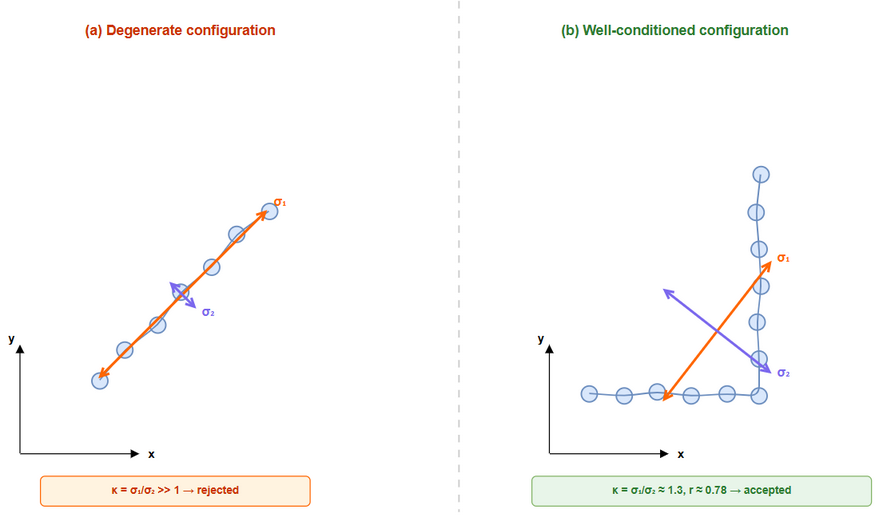
\includegraphics[width=0.85\linewidth]{3-SLAM/3-methodology/figures/geometry-quality}
    \caption{Planar geometry quality assessment for two trajectory configurations.
    \textbf{(a)}~Near-collinear configuration: points lie along a single direction,
    yielding a large condition number $\kappa \gg 1$, indicating insufficient geometric
    spread for reliable plane estimation.
    \textbf{(b)}~Well-conditioned configuration: an L-shaped trajectory distributes
    points across two directions, yielding $\kappa \approx 1.3$ and $r \approx 0.78$.
    Orange and purple arrows denote the first and second principal variance directions
    ($\sigma_1$, $\sigma_2$) obtained from SVD of the centred point set; their
    orientations reflect directions of maximum and minimum variance across all points
    and are not constrained to align with individual path segments.}
    \label{fig:geometry-quality}
\end{figure}

\subsection{GLIM Reference Frame Alignment with Local ENU}

Given two corresponding point sets $\{\mathbf{a}_i\}_{i=1}^N, \{\mathbf{b}_i\}_{i=1}^N \subset \mathbb{R}^3$, the goal is to estimate a rigid-body transformation $(\mathbf{R}, \mathbf{t}) \in \mathrm{SO}(3) \times \mathbb{R}^3$ that minimises the sum of squared alignment errors as defined in the following objective function:
\begin{equation}
\label{eq:kabsch_objective}
\min_{\mathbf{R}, \mathbf{t}} \sum_{i=1}^{N} \left\| \mathbf{b}_i - (\mathbf{R}\mathbf{a}_i + \mathbf{t}) \right\|^2, \quad \text{s.t. } \det(\mathbf{R}) = 1.
\end{equation}

First, the centroids of both point sets are computed as:
\begin{equation}
\label{eq:centroids}
\boldsymbol{\mu}_A = \frac{1}{N} \sum_{i=1}^N \mathbf{a}_i, \qquad \boldsymbol{\mu}_B = \frac{1}{N} \sum_{i=1}^N \mathbf{b}_i.
\end{equation}

The point sets are then centred by subtracting their respective centroids:
\begin{equation}
\label{eq:centering}
\tilde{\mathbf{a}}_i = \mathbf{a}_i - \boldsymbol{\mu}_A, \qquad \tilde{\mathbf{b}}_i = \mathbf{b}_i - \boldsymbol{\mu}_B.
\end{equation}

A $3 \times 3$ cross-covariance matrix $\mathbf{H}$ is formed as:
\begin{equation}
\label{eq:cross_covariance}
\mathbf{H} = \sum_{i=1}^N \tilde{\mathbf{b}}_i \tilde{\mathbf{a}}_i^{\top}.
\end{equation}

The singular value decomposition (SVD) of $\mathbf{H}$ is computed in Equation \eqref{eq:kabsch_svd}:
\begin{equation}
\label{eq:kabsch_svd}
\mathbf{H} = \mathbf{U} \boldsymbol{\Sigma} \mathbf{V}^{\top}.
\end{equation}

To ensure a proper rotation and avoid reflections, a diagonal correction matrix $\mathbf{D}$ is introduced:
\begin{equation}
\label{eq:reflection_correction}
\mathbf{D} = \mathrm{diag}(1,\,1,\,\mathrm{sign}(\det(\mathbf{U}\mathbf{V}^{\top}))).
\end{equation}

The optimal rotation $\mathbf{R}$ is then given by:
\begin{equation}
\label{eq:optimal_rotation}
\mathbf{R} = \mathbf{U}\mathbf{D}\mathbf{V}^{\top}.
\end{equation}

Finally, the translation $\mathbf{t}$ is recovered according to Equation \eqref{eq:recovered_translation}:
\begin{equation}
\label{eq:recovered_translation}
\mathbf{t} = \boldsymbol{\mu}_B - \mathbf{R}\boldsymbol{\mu}_A.
\end{equation}

The resulting rigid transformation $(\mathbf{R}, \mathbf{t})$ aligns the source point set to the target point set in a least-squares sense, as illustrated in \cref{fig:kabsch-alignment}. This static transformation is published to the ROS2 transform tree \cite{macenskiRobotOperatingSystem2022} to link the local ENU frame to the GLIM mapping frame.

\begin{figure}[htbp]
    \centering
    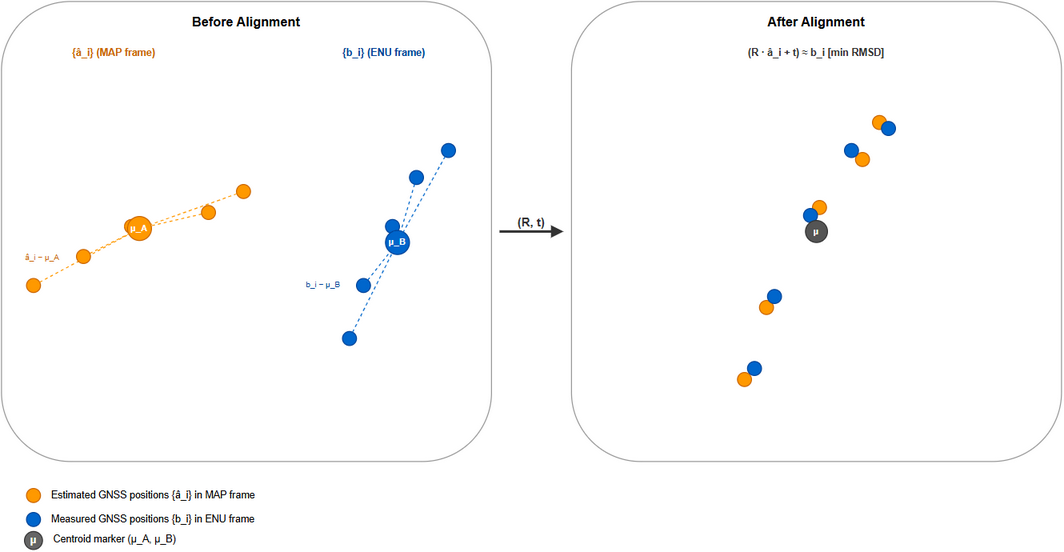
\includegraphics[width=\linewidth]{3-SLAM/3-methodology/figures/kabsch-alignment}
    \caption{Kabsch point-set alignment between estimated GNSS antenna positions $\{\hat{\mathbf{a}}_i\}$ in the MAP frame (orange) and measured GNSS positions $\{\mathbf{b}_i\}$ in the ENU frame (blue). \textit{Left}: before alignment, dashed lines show the centred vectors $\hat{\mathbf{a}}_i - \boldsymbol{\mu}_A$ and $\mathbf{b}_i - \boldsymbol{\mu}_B$ relative to their respective centroids. The clearly different orientations of the two point sets illustrate that the estimated transformation $(\mathbf{R}, \mathbf{t})$ must account for both a rotation and a translation (Equations~\eqref{eq:kabsch_objective}--\eqref{eq:recovered_translation}). \textit{Right}: after alignment, the transformed MAP-frame positions $\mathbf{R}\hat{\mathbf{a}}_i + \mathbf{t}$ coincide with the ENU measurements up to a small residual.}
    \label{fig:kabsch-alignment}
\end{figure}

\subsection{GNSS Prior Factor Construction}

This procedure augments an existing SLAM factor graph \cite{grisettiTutorialGraphBasedSLAM2010a} with GNSS-based prior constraints that relate submap poses to global position measurements. Each GNSS measurement is incorporated as a probabilistic constraint on the estimated submap pose through a known sensor extrinsic calibration.

Let $\mathbf{T}_{\text{map}}^{\text{enu}} \in SE(3)$ denote the rigid transformation from the local ENU frame to the GLIM map frame, and $\mathbf{p}_{\text{imu}}^{\text{gps}} \in \mathbb{R}^3$ the fixed translation from the IMU frame to the GNSS antenna frame. For each correspondence between a submap and a GNSS measurement, the following steps are performed.

First, the GNSS position $\mathbf{p}_{\text{enu}} \in \mathbb{R}^3$ is extracted in the ENU frame and transformed into the map frame as shown in Equation \eqref{eq:enu_to_map}:
\begin{equation}
\label{eq:enu_to_map}
\mathbf{p}_{\text{map}} = \mathbf{T}_{\text{map}}^{\text{enu}} \, \mathbf{p}_{\text{enu}}.
\end{equation}

Next, a diagonal Gaussian noise model is constructed from the reported GNSS covariance. Let $\boldsymbol{\sigma} \in \mathbb{R}^3$ denote the standard deviations obtained from the square root of the covariance diagonal. These values are scaled by a configurable factor $\alpha$ and converted to a covariance matrix in Equation \eqref{eq:gps_noise}:
\begin{equation}
\label{eq:gps_noise}
\boldsymbol{\Sigma}_{\text{gps}} = \mathrm{diag}\!\left((\alpha \boldsymbol{\sigma})^2\right).
\end{equation}

Given a submap pose $\mathbf{T}_{\text{map}}^{\text{sub}} \in SE(3)$, the predicted GNSS antenna position in the map frame is expressed in Equation \eqref{eq:predicted_gps}:
\begin{equation}
\label{eq:predicted_gps}
\hat{\mathbf{p}}_{\text{map}} = \mathbf{T}_{\text{map}}^{\text{sub}} \, \mathbf{p}_{\text{imu}}^{\text{gps}}.
\end{equation}
This formulation is valid as the GLIM submap origin is defined at the IMU center, such that the extrinsic offset $\mathbf{p}_{\text{imu}}^{\text{gps}}$ represents the antenna position relative to the submap origin. An expression-based factor is then constructed to minimize the residual between the predicted and measured positions under the noise model $\mathcal{N}(\mathbf{0}, \boldsymbol{\Sigma}_{\text{gps}})$:
\begin{equation}
\label{eq:gnss_factor}
\mathbf{r}(\mathbf{T}_{\text{map}}^{\text{sub}}) = \left\| \hat{\mathbf{p}}_{\text{map}} - \mathbf{p}_{\text{map}} \right\|^2_{\boldsymbol{\Sigma}_{\text{gps}}}.
\end{equation}

This factor directly constrains the corresponding submap pose variable in the factor graph, contributing to global consistency and LiDAR-inertial odometry drift correction. In effect, this factor constrains the GLIM-predicted position of the GPS antenna using the measured GNSS position at that time. \cref{fig:factor-graph} depicts the resulting factor graph structure, highlighting the asynchronous attachment of GNSS prior factors to submap pose nodes alongside the continuous LiDAR--IMU odometry chain.

\begin{figure}[htbp]
    \centering
    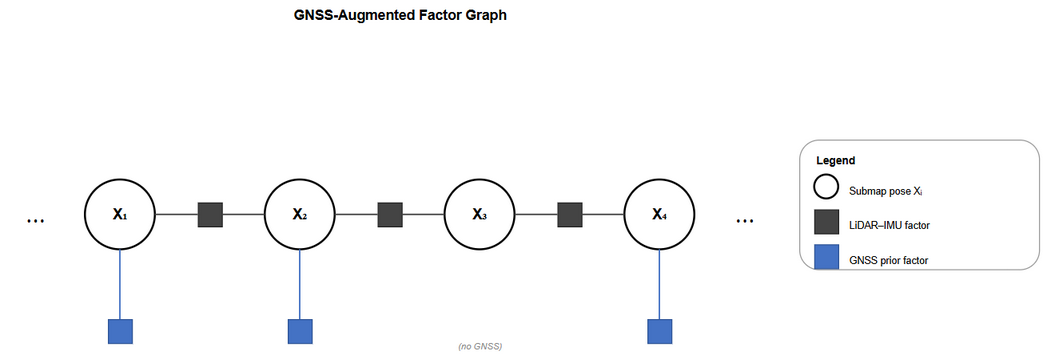
\includegraphics[width=0.85\linewidth]{3-SLAM/3-methodology/figures/factor-graph}
    \caption{GNSS-augmented factor graph structure. Circles denote submap pose variables $X_i$; dark squares represent LiDAR--IMU odometry factors between consecutive submaps; blue squares represent GNSS prior factors attached to corresponding submap poses. GNSS measurements arrive asynchronously and are therefore not associated with every submap (illustrated by the absent factor at $X_3$).}
    \label{fig:factor-graph}
\end{figure}

\subsection{Robust SLAM Parameterisation via Iterative Region Refinement}

The optimisation of Simultaneous Localisation and Mapping (SLAM) parameters is a high-dimensional, non-convex problem where the objective is to identify a parameter vector $\Theta$ that minimises localisation error across heterogeneous environments \cite{hanMultiObjectiveOptimizationLoop2020}. This subsection proposes a model-free, heuristic region-refinement algorithm that transitions from global stochastic exploration to localised deterministic refinement. The strategy assumes that optimal configurations cluster within specific sub-regions of the hyper-dimensional search space $\Omega$, which are iteratively identified and contracted using statistical distribution analysis.

\subsubsection{Problem Formulation}
We define the SLAM system as a complex function $f(X,\theta)$, where $X$ represents raw sensor data (e.g., LiDAR scans and inertial measurements) and $\Theta$ is the $d$-dimensional parameter vector. In a typical LiDAR-inertial setup, $\Theta$ includes parameters such as LiDAR resolution and registration strategy. The objective is to find $\Theta^*$ such that:
\begin{equation}
    \Theta^* = \arg\min_{\Theta \in \Omega} \mathcal{J}(\Theta)
\end{equation}
where $\mathcal{J}$ is a robust objective function representing the consensus performance across $K$ distinct motion profiles.

\subsubsection{Sampling via Latin Hypercube Strategy}
To explore the initial parameter manifold, we utilise Latin Hypercube Sampling (LHS) as an alternative to traditional grid search or independent Monte Carlo (MC) sampling \cite{deutschLatinHypercubeSampling2012}. LHS is technically categorised as a stratified sampling design \cite{chrismanLatinHypercubeSampling2014}. For a sample size $N$ in $d$ dimensions, the range of each parameter $\theta_j$ is partitioned into $N$ equiprobable intervals for $j=1, \dots, d$ \cite{chrismanLatinHypercubeSampling2014}. The mathematical constraint --- ensuring exactly one sample per row and column of the grid --- minimises the ``clustering'' phenomenon common in pure random sampling \cite{deutschLatinHypercubeSampling2012}. This stratification ensures that the marginal distribution of each parameter is sampled uniformly, achieving a lower variance than independent Monte Carlo sampling for the same sample size \cite{packhamLatinHypercubeSampling2008}.

\paragraph{Implementation and Normalisation}
Parameter vectors are first normalised to the unit hypercube $[0, 1]^d$ \cite{deutschLatinHypercubeSampling2012}. To ensure reproducibility, the pseudo-random permutations used to construct the hypercube are seeded deterministically. The samples are subsequently scaled to physical ranges using:
\begin{equation}
    \theta_{j,i} = \theta_{j, \min} + u_{j,i} (\theta_{j, \max} - \theta_{j, \min})
\end{equation}
where $\theta_{j, \min}$ and $\theta_{j, \max}$ represent the physical lower and upper bounds for parameter $j$.

\subsubsection{The Multi-Dataset Consensus Framework}
A primary challenge in SLAM optimisation is the risk of ``over-specialisation'', where parameters become overfitted to the unique noise characteristics of a single trajectory \cite{soaresVARSLAMVisualAdaptive2025}. We implement a Consensus Survival Framework to prioritise reliability across datasets.

In some situations, standard ``Mean-Performance Optimisation'' can hide brittle configurations that perform well on average but fail catastrophically on a single sequence \cite{kandasamyTuningHyperparametersGrad}. However, in this setting, catastrophic failure typically results in excessively high amplitude errors, which effectively inflate the mean normalised error. That being said, some particular parameter configurations can lead to excessive GPU draw, resulting in a runtime CUDA out-of-memory error. If the parameter set does not complete processing the trajectory on any dataset $k$, it is assigned an infinite cost and discarded from the survivor pool. This ensures the survival of only those configurations that meet the computational requirements of the system.

\paragraph{Formal Objective Function}
For the "surviving" configurations, the objective function $J(\theta)$ is defined as the mean normalized error across the valid sequences \eqref{eq:piecewise_success}:
\begin{equation}
\label{eq:piecewise_success}
J(\theta) = 
\begin{cases} 
\frac{1}{K} \sum_{k=1}^K E_k(\theta) & \text{if success} \in \{D_1, \dots, D_K\} \\ 
\infty & \text{otherwise} 
\end{cases}
\end{equation}

where $E_k(\theta)$ is the primary performance metric for dataset $k$.

\subsubsection{Iterative Region Refinement (IRR)}
The optimisation proceeds through an ``Iterative Contraction'' or ``Funnel'' strategy. This mirrors the reduction of a search radius in traditional Trust Region Methods \cite{nocedalTrustRegionMethods2006}, concentrating the sampling density into the most promising basins of attraction.

\paragraph{Statistical Search Space Contraction}
At the conclusion of each phase $i$, the top-performing configurations are used to calculate new search boundaries for phase $i+1$. We employ the 10th and 90th percentiles of the elite set as robust estimators for the update rule in Equation \eqref{eq:quantile_update}:
\begin{equation}
\label{eq:quantile_update}
\Omega_{j, i+1} = [P_{10}(\theta_{j, \text{top}}), P_{90}(\theta_{j, \text{top}})].
\end{equation}
This quantile-based reduction is superior to using absolute Min/Max values because it is resilient to ``lucky'' outliers --- configurations that may perform well due to noise interactions rather than parameter stability.

\paragraph{Refinement Phase Schedule}
The optimisation is structured into four phases, increasing the selection pressure (lower survival rate) as the search space contracts, as detailed in \cref{tab:phases}:

\begin{table}[h]
\centering
\caption{Evolutionary Phases of the Sampling Algorithm}
\label{tab:phases}
\begin{tabularx}{\textwidth}{@{} l l c c X @{}}
\toprule
\textbf{Phase} & \textbf{Objective} & \textbf{Iterations (N)} & \textbf{Survival Rate} & \textbf{Description} \\ \midrule
Phase 1 & Thinning & 100 & 30\% & Broad exploration identifying stable regions. \\
Phase 2 & Narrowing & 100 & 20\% & Convergence on local minima. \\
Phase 3 & Refinement & 100 & 10\% & High-density sampling within basins. \\
Phase 4 & Fine-tuning & 75 & 1.3\% & Final tuning to find top candidate. \\ \bottomrule
\end{tabularx}
\end{table}

This incremental strategy is distinct from Successive Halving (SHA) \cite{jamiesonNonstochasticBestArm2015}, as it preserves a continuous distribution of potential solutions rather than discarding them in discrete early-stopping steps, which is critical for SLAM where early performance does not always correlate with final drift. \cref{fig:irr-funnel} visualises the contracting search space across phases, showing how sample density converges toward the optimal configuration.

\begin{figure}[htbp]
    \centering
    \begin{subfigure}[t]{0.57\textwidth}
        \centering
        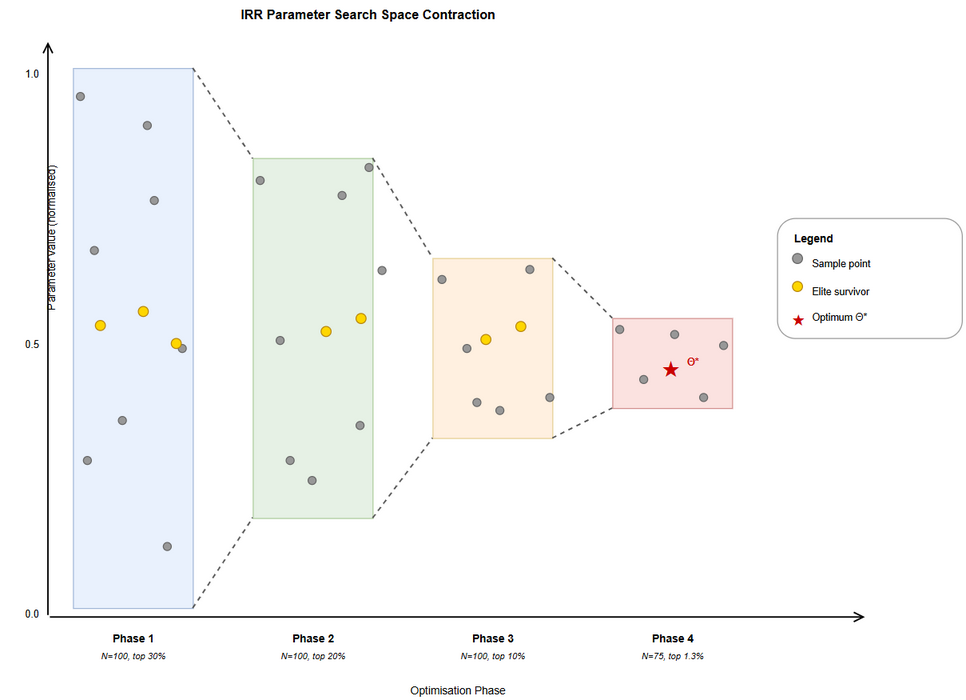
\includegraphics[width=\linewidth]{3-SLAM/3-methodology/figures/irr-funnel}
        \caption{Parameter search space contraction across four optimisation phases. Each coloured band represents the active search bounds for a single parameter dimension (normalised to $[0,1]$); bounds are updated between phases using the $P_{10}$--$P_{90}$ range of the elite survivor set (dashed diagonal lines). Grey dots are sampled configurations; gold dots are elite survivors; the red star marks the final optimum $\Theta^*$.}
        \label{fig:irr-funnel}
    \end{subfigure}
    \hfill
    \begin{subfigure}[t]{0.40\textwidth}
        \centering
        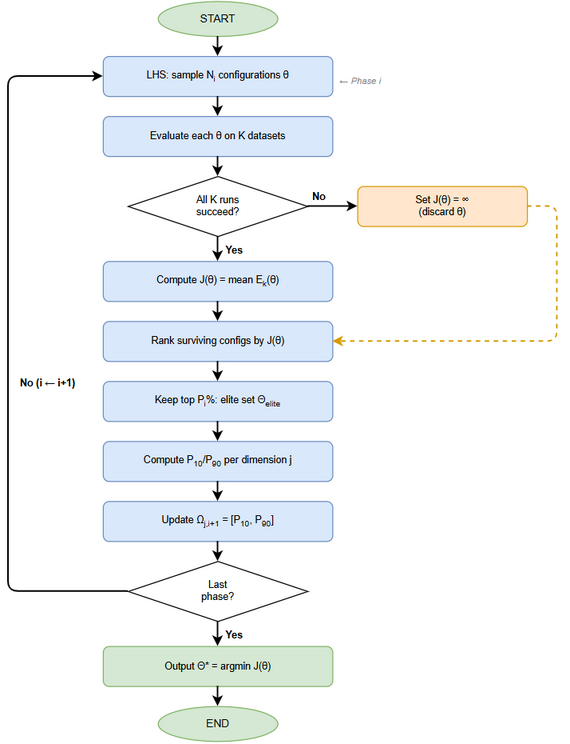
\includegraphics[width=\linewidth]{3-SLAM/3-methodology/figures/irr-flowchart}
        \caption{Algorithmic flowchart of the IRR procedure. Each phase samples $N_i$ configurations via LHS, evaluates them on $K$ datasets, discards failures (cost $= \infty$), ranks survivors by $J(\theta)$, retains the elite top $P_i\%$, and contracts the search bounds $\Omega_{j,i+1}$ using the $P_{10}$--$P_{90}$ quantile range.}
        \label{fig:irr-flowchart}
    \end{subfigure}
    \caption{IRR optimisation strategy: \subref{fig:irr-funnel}~contracting parameter search space across phases; \subref{fig:irr-flowchart}~per-phase algorithmic procedure.}
    \label{fig:irr}
\end{figure}

\subsubsection{Optimisation Metrics}

For the optimisation of the base GLIM algorithm, the cost function for candidate ranking is the Trajectory Error Percentage ($TEP$), calculated as the percentage of the ratio of Absolute Trajectory Error ($ATE$) \cite{sturmBenchmarkEvaluationRGBD2012} to the total trajectory length ($L$):
\begin{equation}
\label{eq:tep}
TEP = \frac{ATE}{L} \times 100\%.
\end{equation}
The $TEP$ effectively measures the per cent drift per metre of motion.

For the optimisation of the proposed method, the cost function is a custom metric referred to as Global Alignment and Smoothness Profile ($GASP$). This is calculated by taking the weighted sum of the $ATE$ per metre and the standard deviation of the translational Relative Pose Error ($RPE$), as defined in Equation \eqref{eq:gasp}:
\begin{equation}
\label{eq:gasp}
\text{GASP} = w_{\text{drift}} \cdot \left( \frac{ATE}{L} \right) + w_{\text{smoothness}} \cdot \text{Translational RPE}.
\end{equation}
The weights $w_{\text{drift}}$ and $w_{\text{smoothness}}$ have been empirically tuned such that each term contributes approximately equally to the total cost. Because the weighted sum mixes quantities with different units, GASP serves as a relative performance index; its values are meaningful only when compared within the same experimental framework.

\subsection{Experimental Setup}
\label{subsec:slam-experimental-setup}

The following subsection describes the datasets and evaluation protocol used to assess the methods presented above.

\subsubsection{Parameterisation Datasets}

Five datasets were used to parameterise the two optimised configurations — the refined GLIM algorithm and the proposed GNSS-augmented method. The datasets span two distinct agricultural environments: one apple orchard (Dataset~1) and four vineyard traversals (Datasets~0, 2, 3, and~4), the latter all collected at the same farm. This environmental diversity was deliberate, as including a structurally different environment reduces the risk that the parameterised configurations are over-specialised to a single terrain type.

\begin{itemize}
  \item \textbf{Dataset~0 --- Vineyard.} A forward-and-return traversal. The altitude increases gradually on the forward pass and decreases correspondingly on the return.
  \item \textbf{Dataset~1 --- Apple orchard.} A forward-and-return traversal of an apple orchard. The altitude profile is more complex than the vineyard datasets, featuring substantially more localised elevation dips and bumps throughout, making this dataset the most challenging for vertical estimation.
  \item \textbf{Dataset~2 --- Vineyard.} A single-direction traversal with no return pass, starting from the opposite end of the vineyard row relative to all other vineyard datasets. The altitude decreases gradually over the course of the traversal — the inverse of the profile observed in Datasets~0, 3, and~4.
  \item \textbf{Dataset~3 --- Vineyard.} A forward-and-return traversal at the same farm as Datasets~0, 2, and~4. The altitude profile follows the same gradual increase--decrease pattern as Datasets~0 and~4.
  \item \textbf{Dataset~4 --- Vineyard.} A forward-and-return traversal at the same farm as Datasets~0, 2, and~3, with the same altitude profile as Datasets~0 and~3.
\end{itemize}

\subsubsection{Evaluation Dataset}

The Evaluation Dataset is a held-out vineyard traversal that was not used at any stage of the parameterisation process. It was collected at the same farm as Datasets~0, 2, 3, and~4, but follows a distinct route not present in the parameterisation data. The altitude profile is consistent with that of Datasets~0, 1, 3, and~4: a gradual increase on the forward traversal and a corresponding decrease on the return. The dataset may differ from the parameterisation datasets in GNSS coverage and signal conditions, depending on the canopy density and geometry of the specific route.

The purpose of this dataset is to provide an unbiased estimate of whether the performance improvements observed during parameterisation reflect genuine algorithmic improvement, or whether they are artefacts specific to the routes on which parameters were tuned.

\subsubsection{Evaluation Protocol}

Three configurations were evaluated: the baseline GLIM algorithm, the refined GLIM algorithm with optimised parameters, and the proposed GNSS-augmented method. Each configuration was evaluated on each of the five parameterisation datasets using a single run per dataset.

For the Evaluation Dataset, each configuration was evaluated across five independent runs. This repetition is motivated by the non-deterministic behaviour of the SLAM system: internal parallelism and floating-point operation ordering cause run-to-run variation in the generated trajectory, even under identical input conditions. A single run on an unseen dataset therefore risks reporting an uncharacteristic outcome. For each metric, the mean, standard deviation, median, minimum, and maximum across the five runs are reported.

Performance is assessed using the metrics defined in \cref{sec:slam-methodology}: RMSE (per axis and aggregate 3D), ATE, maximum 3D positional error, error per metre, error percentage per metre, RPE at displacement intervals of 1\,m and 10\,m (RMSE, mean, standard deviation, and maximum translation error), and, for the proposed method, GASP.

